\chapter{Signal Chain%
  \label{chap:\currfilebase}}

Some sensors operate at small energies. The signals are to weak to be converted into digital ones by standard components. \emph{Signal conditioning} enables us to amplify and denoise analog signals so that the signal can be further processed. In our application, both the load cell's and accelerometer's senors signal must be amplified to match the input range of the respective \ac{ADC}. In this section we put together all conditioning steps necessary from sensor to the digital signal under the term signal chain. Because the selected accelerometers come in an \ac{IC} packages that include the complete signal chain, we focus on the signal chain of the load cell. For more background on signal conditioning and processing, read \secref{signal_conditioning_processing}.

\section{Excitation}

\section{Amplification}
Electrical signals are amplified by active electrical components; i.e.\ typically by \ac{OPA}s or circuits of \ac{OPA}s.

\subsection{Operational Amplifier}

Amplifiers apply signal gain on electrical inputs so that the output matches the input times a constant gain factor. The latter is determined by the impedance of the subsequent device in the signal chain and the magnitude at the input. But by setting the gain factor one predetermines the introduced absolute noise due to the amplifier's inherent \ac{SNR}.

In simple amplifiers, the \ac{SNR} purely depends on the quality of the components and the environmental conditions. This can be bypassed by building differential setups, where amplifiers, like transistors and field transistors, are fed with both the non-inverted and the inverted input signal individually. With multi-staging and additional filter circuits one can reduce the noise further and ultimately the \ac{SNR} becomes strongly dependent on the circuit design and less dependent on the quality of each component. Specific to different applications, many variants of the described circuitry are available in so-called Operational Amplifiers (\acs{OPA}s).

\ac{OPA}s are available in a variety of \ac{IC} packages and differ little from discrete transistors in terms of size and prize. In some packages even multiple individual \ac{OPA}s are included. Initially \ac{OPA}s offered high accuracy at low frequencies. Over time different circuit designs for different needs have broadened the field of application considerably. Today, it is hard to find a task that is better met by a transistor than by an \ac{OPA}. We subdivide the latter into four main types, as shown in \figref{fig:op_amp_types}. The differences are high-resistive or low-resistive inputs and outputs. The standard \ac{OPA} and the transconductance amplifier, for example, have high-resistance inputs. Therefore, they are voltage controlled. The outputs on the other hand are of low and high internal resistance respectively, where low-resistance outputs act as voltage sources and high-resistance outputs act as current sources. In the naming convention the two leading letters represent input and output. ``V'' at first position stands for a voltage controlled \ac{OPA} with a high-resistance input, where ``C'' means current controlled and low-resistive input. At the second position ``V'' and ``C'' define low- and high-resistance outputs that act as voltage and current source respectively.
The differential gain of an ideal VV-\ac{OPA} is given by the slope at the operating b by
\begin{align}
  A_D &= \eval{\dv{V_o}{V_D}}_{b}
\end{align}


Because of their differential circuit, \ac{OPA}s normally are powered by symmetric operating voltages. Rail-to-rail \ac{OPA}s have the capability to control the output between the positive and negative supply voltage, allowing maximal amplification, see \figref{fig:plot_opamp_railrail}.
When working with digital circuits, a single voltage supply is preferred. For this case, single supply voltage \ac{OPA}s are used.

\begin{figure}[!htb]
  \sbox0{\subcaptionbox{Amplifier with voltage output\label{sfig:op_amp_transfer_volt}}{%
      \includegraphics[scale=0.72]{figures/electronics/op_amp/op_amp_transfer_volt}
    }}% a
  \sbox1{\subcaptionbox{Amplifier with current output\label{sfig:op_amp_transfer_curr}}{%
    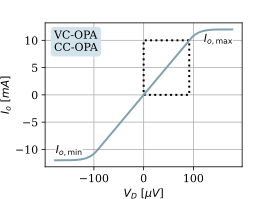
\includegraphics[scale=0.72]{figures/electronics/op_amp/op_amp_transfer_curr}
    }}% b
  \centering
  {%
    \renewcommand{\arraystretch}{6}%
    \setlength{\tabcolsep}{0em}
    \begin{tabular}{ccc}
      \usebox0 & \usebox1 \\
    \end{tabular}%
  }
  \caption[Capacitive displacement sensors]{Capacitive displacement sensors \cite{webster2018measurement}%
    \label{fig:cap_disp}}
\end{figure}

\begin{figure}[htb!]
  \centering
  \includegraphics[scale=1]{figures/electronics/op_amp/op_amp_types/op_amp_types}
  \caption[Main OPA types]{Main operational amplifier types%
  \label{fig:op_amp_types}}
\end{figure}

\begin{figure}[htb!]
  \centering
  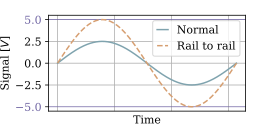
\includegraphics[scale=0.72]{figures/electronics/op_amp/plot_opamp_railrail}
  \caption[OPA controllability]{OPA controllability at $\pm\SI{5}{\volt}$ operating voltage%
    \label{fig:plot_opamp_railrail}}
\end{figure}

\section{Filtering}

Whenever we measure a signal in the real world, it will inherently contain some form of noise. Filtering enables us to cut off contributions to the signal amplitude, that are outside the expected signal frequency bandwidth.

The two main types of filters are analog and digital ones, where the digital filters are more versatile, cost-effective and precise compared to their counterpart. Nevertheless, analog filters are required when filtering analog signals, i.e.\ whenever the signal must be denoised or bandwidth limited. As an example, it is advantageous if a signal is denoised, before it is amplified because we do not want to amplify the noise components of the signal. Furthermore electric devices in the signal chain have a bandwidth limited range of operation. Disturbances of the signal occur due to frequency dependent phase shifts or damping when operating outside these ranges. Namely when digitizing a signal, the additional effect of aliasing may disturb a signal significantly if it contains frequency components above the Nyquist frequency.

\section{Analog to Digital Conversion}

Additionally to other noise sources in the signal chain the \ac{ADC} shows internal noise that can categorized into two uncorrelated main sources. The quantization noise and the thermal noise. The total internal noise can thus be expressed as the Euclidean norm of these two sources.

\begin{align}
  n_\text{ADC} &= \sqrt{n_{\text{ADC},\text{Thermal}}^2 + n_{\text{ADC},\text{Quantization}}^2}
\end{align}

Quantization noise is present due to the process of mapping an infinite number of possible electrical signal values in an analog signal to a finite number of digital codes. Subsequently, any digital output corresponds to an infinite number of analog inputs within range of the output value, plus and minus half the \ac{LSB} size, $s_\text{LBS}$. One can decrease quantization noise by choosing a higher resolution \ac{ADC}.

\begin{align}
  s_\text{LBS} &= \frac{V_{FSR}}{2^m}
\end{align}
where
\begin{description}[topsep=0ex, noitemsep]
  \item $V_{\text{FSR}}$ is the full-scale range of the analog input value and
  \item $m$ is the resolution in number of bits
\end{description}

\begin{figure}[!htb]
  \centering
  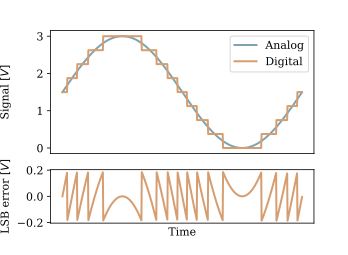
\includegraphics[scale=0.72]{figures/electronics/adc/plot_lsberr}
  \caption[ADC LSB waveform]{\ac{ADC} --- Analog input, digital output and \ac{LSB} error waveform with $s_\text{LBS} = \SI{375}{\milli\volt}$\cite{hall2020fund}%
    \label{fig:plot_lsberr}}
\end{figure}

Thermal noise is a phenomenon inherent in all electrical components. Because of this, it is a function of the device design and cannot be affected by the embedded system designer. Typically, one assumes the thermal noise to have a Gaussian distribution.

\begin{figure}
  \centering
  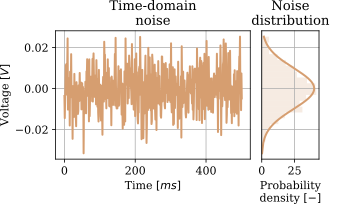
\includegraphics[scale=0.72]{figures/electronics/adc/plot_thermerr}
  \caption[ADC thermal noise]{ADC --- Thermal noise in the time domain with Gaussian probability density~\cite{hall2020fund}%
    \label{fig:plot_themerr}}
\end{figure}
